\subsubsection{Cache Structure}

Each entry (cache line) in the cache includes:
\begin{itemize}
    \item (\textbf{V}) \textbf{Valid bit} to indicate if this position contains valid data or not. At the bootstrap, all the entries in the cache are marked as \texttt{INVALID}.

    \item (\textbf{TAG}) \textbf{Cache Tag(s)} contains the value that univocally identifies the memory address corresponding to the stored data.

    \item (\textbf{DATA}) \textbf{Cache Data} contains a copy of data (block or cache line).
\end{itemize}
\begin{figure}[!htp]
    \centering
    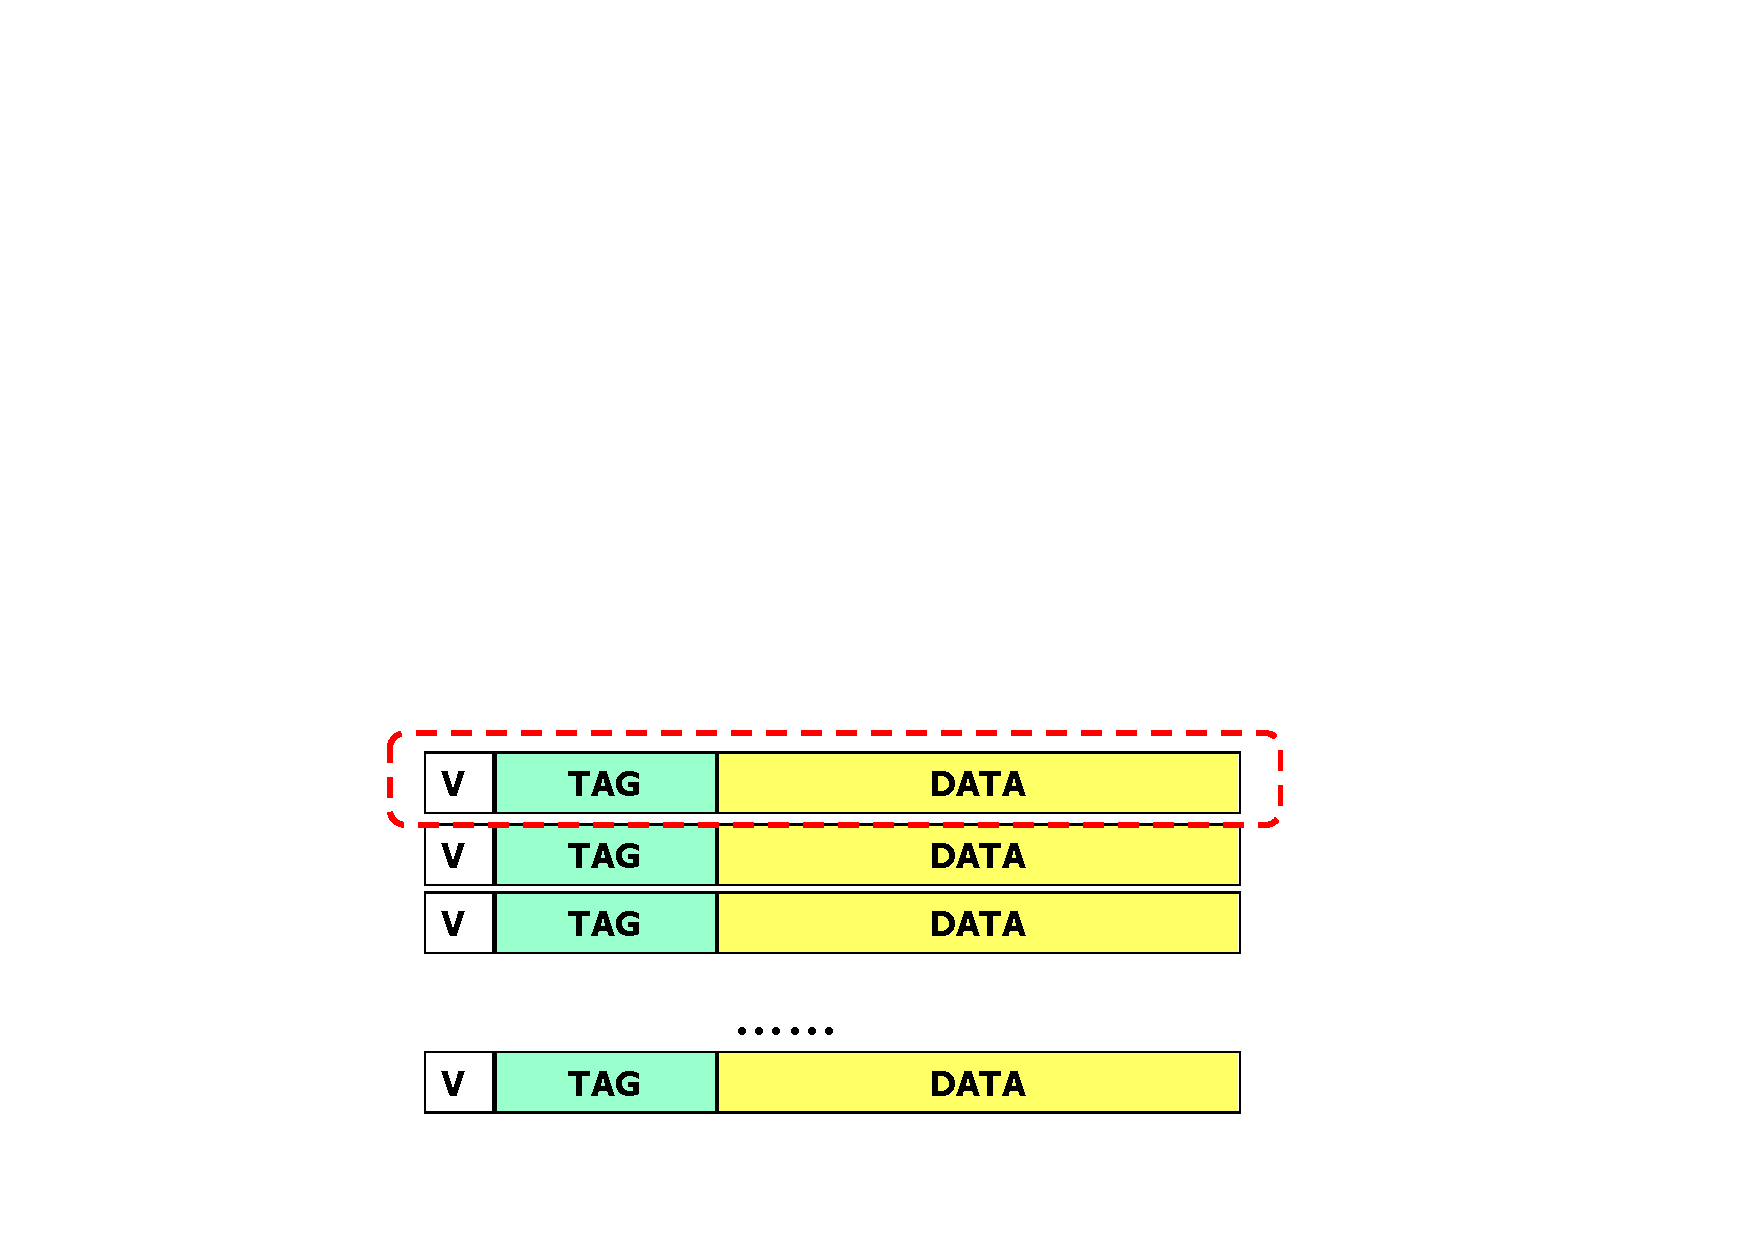
\includegraphics[width=.7\textwidth]{img/cache-structure-1.pdf}
\end{figure}

\noindent
After a general presentation of the cache structure, we answer four questions about the memory hierarchy to understand different topics: 
\begin{itemize}
    \item \textbf{Block placement} (page~\pageref{Block placement}). \emph{Where can a block be placed in the upper level?}
    \begin{itemize}
        \item Direct Mapped Cache (page~\pageref{Direct Mapped Cache})
        \item Fully Associative Cache (page~\pageref{Fully Associative Cache})
        \item \emph{n}-way Set-Associative Cache (page~\pageref{n-way Set-Associative Cache})
    \end{itemize}
    
    \item \textbf{Block identification}. \emph{How is a block found if it is in the upper level?}
    
    \item \textbf{Block replacement}. \emph{Which block should be replaced on a miss?}
    
    \item \textbf{Write strategy}. \emph{What happens on a write?}
\end{itemize}

\newpage

\begin{center}
    \large
    \textcolor{Red2}{\textbf{Block placement}}
    \label{Block placement}
\end{center}

\noindent
The main question is: \emph{where can a block be placed in the upper level?} In other words, the problem is: given the address of the block in the main memory, \textbf{where can the block be placed in the cache}?

\highspace
So, we need to find the \textbf{correspondence between the memory address and the cache address of the block}. This correspondence \textbf{depends on the cache structure} and can be of three types:
\begin{itemize}
    \item \textbf{Direct Mapped Cache}
    \item \textbf{Fully Associative Cache}
    \item \textbf{\emph{n}-way Set-Associative Cache}
\end{itemize}

\subsubsection*{\textcolor{Red2}{Direct Mapped Cache}}\label{Direct Mapped Cache}

With the \definition{Direct Mapped Cache} structure, \textbf{each memory location corresponds to one cache location and only one cache location}. The following formula gives the \textbf{cache address of the block}:
\begin{equation}\label{eq: direct mapped cache}
    \left(\texttt{Block Address}\right)_{\texttt{cache}} = \left(\texttt{Block Address}\right)_{\texttt{mem}} \texttt{mod} \left(\texttt{\# Cache Blocks}\right)
\end{equation}
The \emph{block address} of the \emph{cache} corresponds to the modulo operation between the \emph{block address} of the \emph{memory} and the \emph{number} (\#) \emph{of cache blocks}. The \href{https://en.wikipedia.org/wiki/Modulo}{modulo operation} returns a division's remainder or signed remainder after dividing one number by another.

\begin{figure}[!htp]
    \centering
    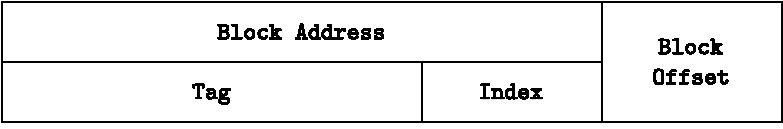
\includegraphics[width=.9\textwidth]{img/direct-mapped-cache-1.pdf}
    \caption{This figure shows the memory address composed of the block address (tag and index used to identify the block) and the block offset.}
    \label{fig: Memory Address - Direct Mapped Cache}
\end{figure}

\noindent
From Figure~\ref{fig: Direct Mapped Cache - Structure}, we can see the complete structure of the cache if we choose the direct mapped cache technique. 

\highspace
The rectangle on the top is the memory address (Figure~\ref{fig: Memory Address - Direct Mapped Cache}). First, we check the \emph{Tag} value; if it's equal to the value in the cache, we check the \emph{Valid bit} (V) to see if the position contains valid data: if the value is 1, we have a cache hit; otherwise, the data is invalid. The \emph{Tag} contains the value that univocally identifies the memory address corresponding to the stored data. To take the \emph{data word}, we use the \emph{block offset} as the \emph{selector} in the \href{https://en.wikipedia.org/wiki/Multiplexer}{multiplexer} to choose which data block to take. The index field indicates the cache row to check.

\newpage

\begin{figure}[!htp]
    \centering
    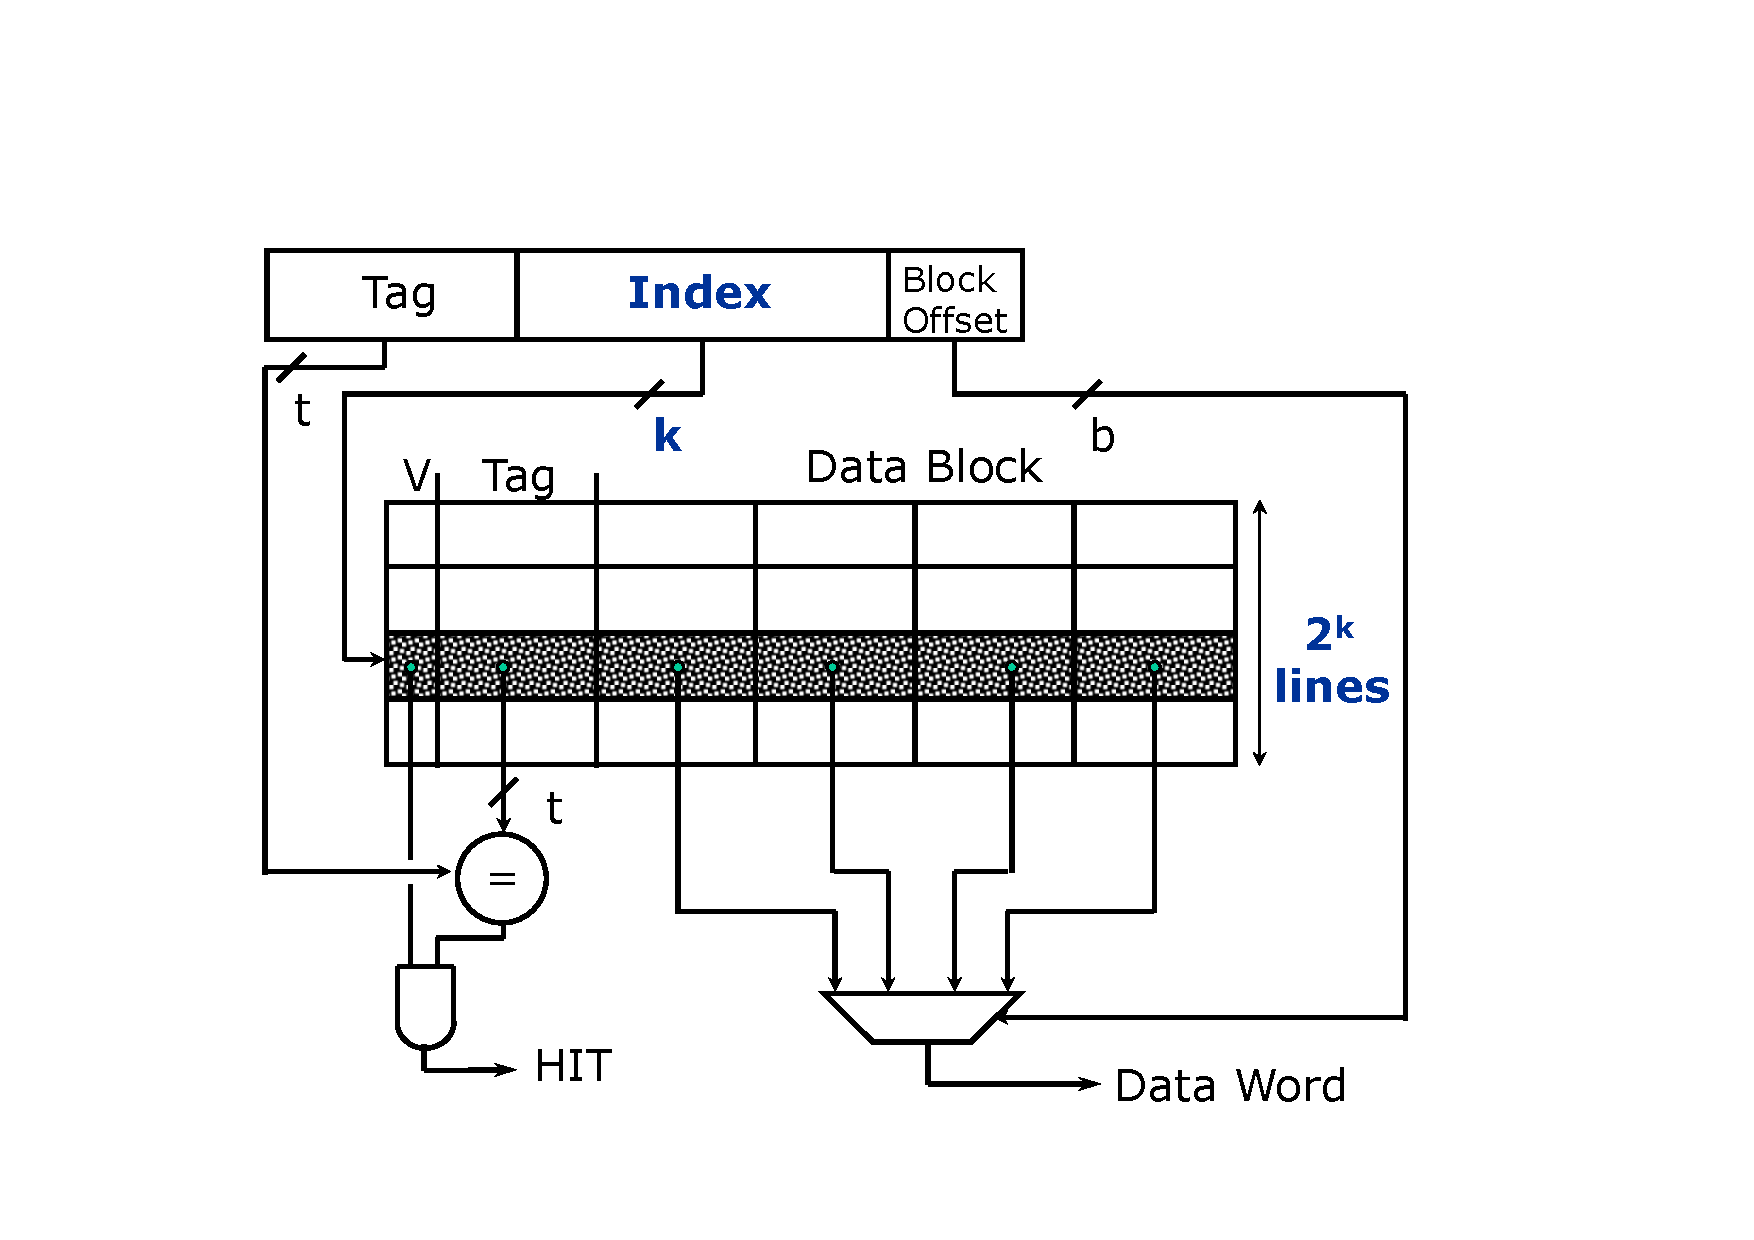
\includegraphics[width=.7\textwidth]{img/direct-mapped-cache-2.pdf}
    \caption{The cache structure of the \emph{Direct Mapped Cache} technique.}
    \label{fig: Direct Mapped Cache - Structure}
\end{figure}

\noindent
For \example{example}, we assume a block-frame address composed of 32 bits. Our cache structure is direct mapped, and the number of cache blocks is 8. A possible exercise could be \textbf{determining where block 12 can be placed in the 8-block cache}.

\highspace
To solve this problem, we can use the formula no \ref{eq: direct mapped cache} on page \pageref{eq: direct mapped cache}: 
\begin{equation*}
    \left(\texttt{Block Address}\right)_{\texttt{cache}} = 12 \mod 8 = 5
\end{equation*}
The result is $5$, so the answer is: with the direct mapped technique, \textbf{the block number is 4} (because the first index of the cache blocks is zero and not 1).

\begin{figure}[!htp]
    \centering
    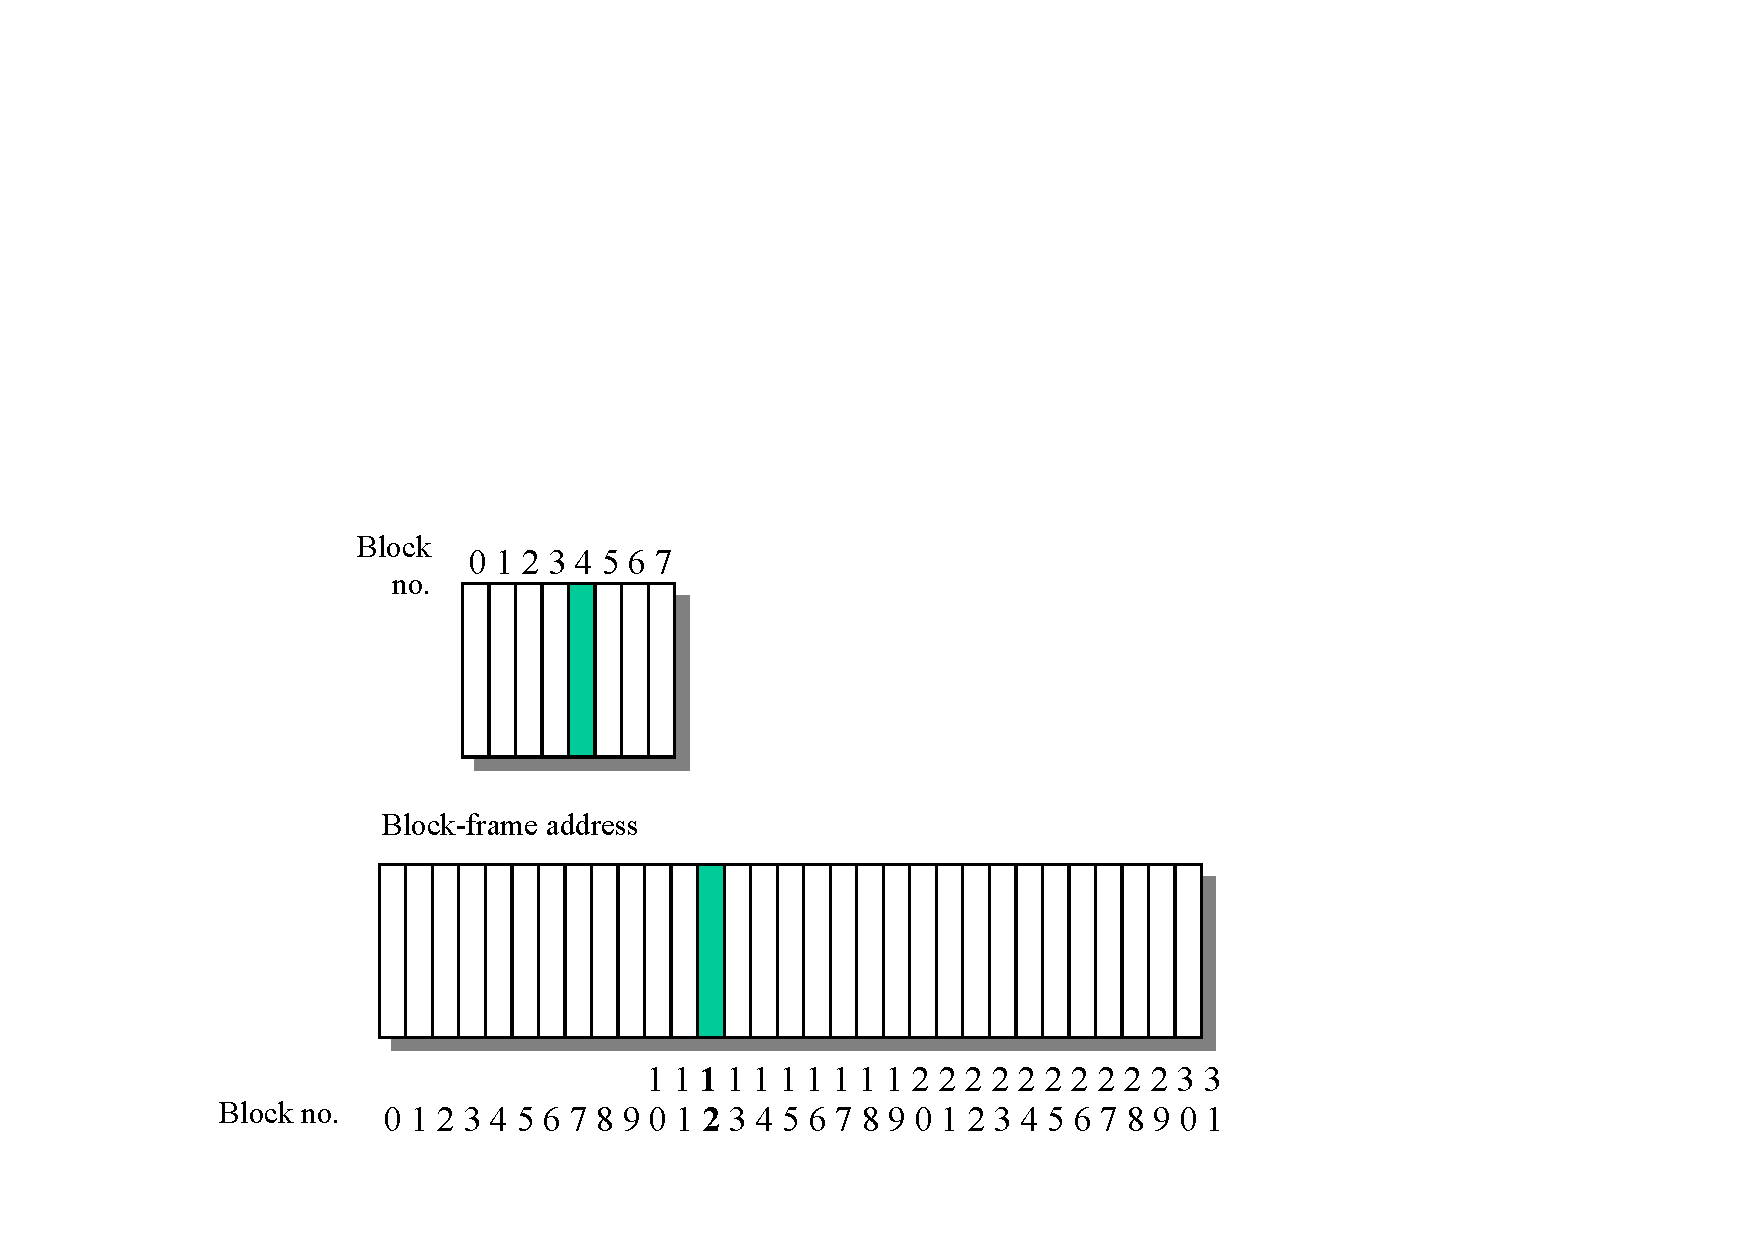
\includegraphics[width=.8\textwidth]{img/direct-mapped-cache-3.pdf}
\end{figure}

\newpage

\subsubsection*{\textcolor{Red2}{Fully Associative Cache}}\label{Fully Associative Cache}

In a \definition{Fully Associative Cache}, the \textbf{memory block can be placed in any position of the cache}. So, all the \textbf{cache blocks must be checked during the search of the block}.

\highspace
Note the \textbf{index does not exist} in the memory address; there are the Tag bits only:
\begin{equation}\label{eq: Fully Associative Cache}
    \texttt{Number of blocks} = \dfrac{\texttt{Cache Size}}{\texttt{Block Size}}
\end{equation}
The Memory Address comprises the Block Address (Tag) and the Block Offset.

\begin{figure}[!htp]
    \centering
    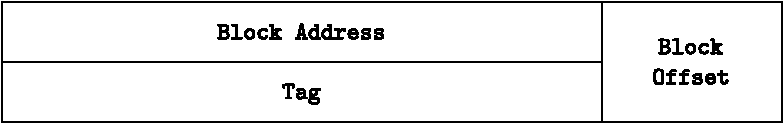
\includegraphics[width=.9\textwidth]{img/fully-associative-cache-1.pdf}
    \caption{The Memory Address comprises the Block Address (Tag) and the Block Offset.}
\end{figure}

\noindent
The structure of the cache using this technique is as follows:

\begin{figure}[!htp]
    \centering
    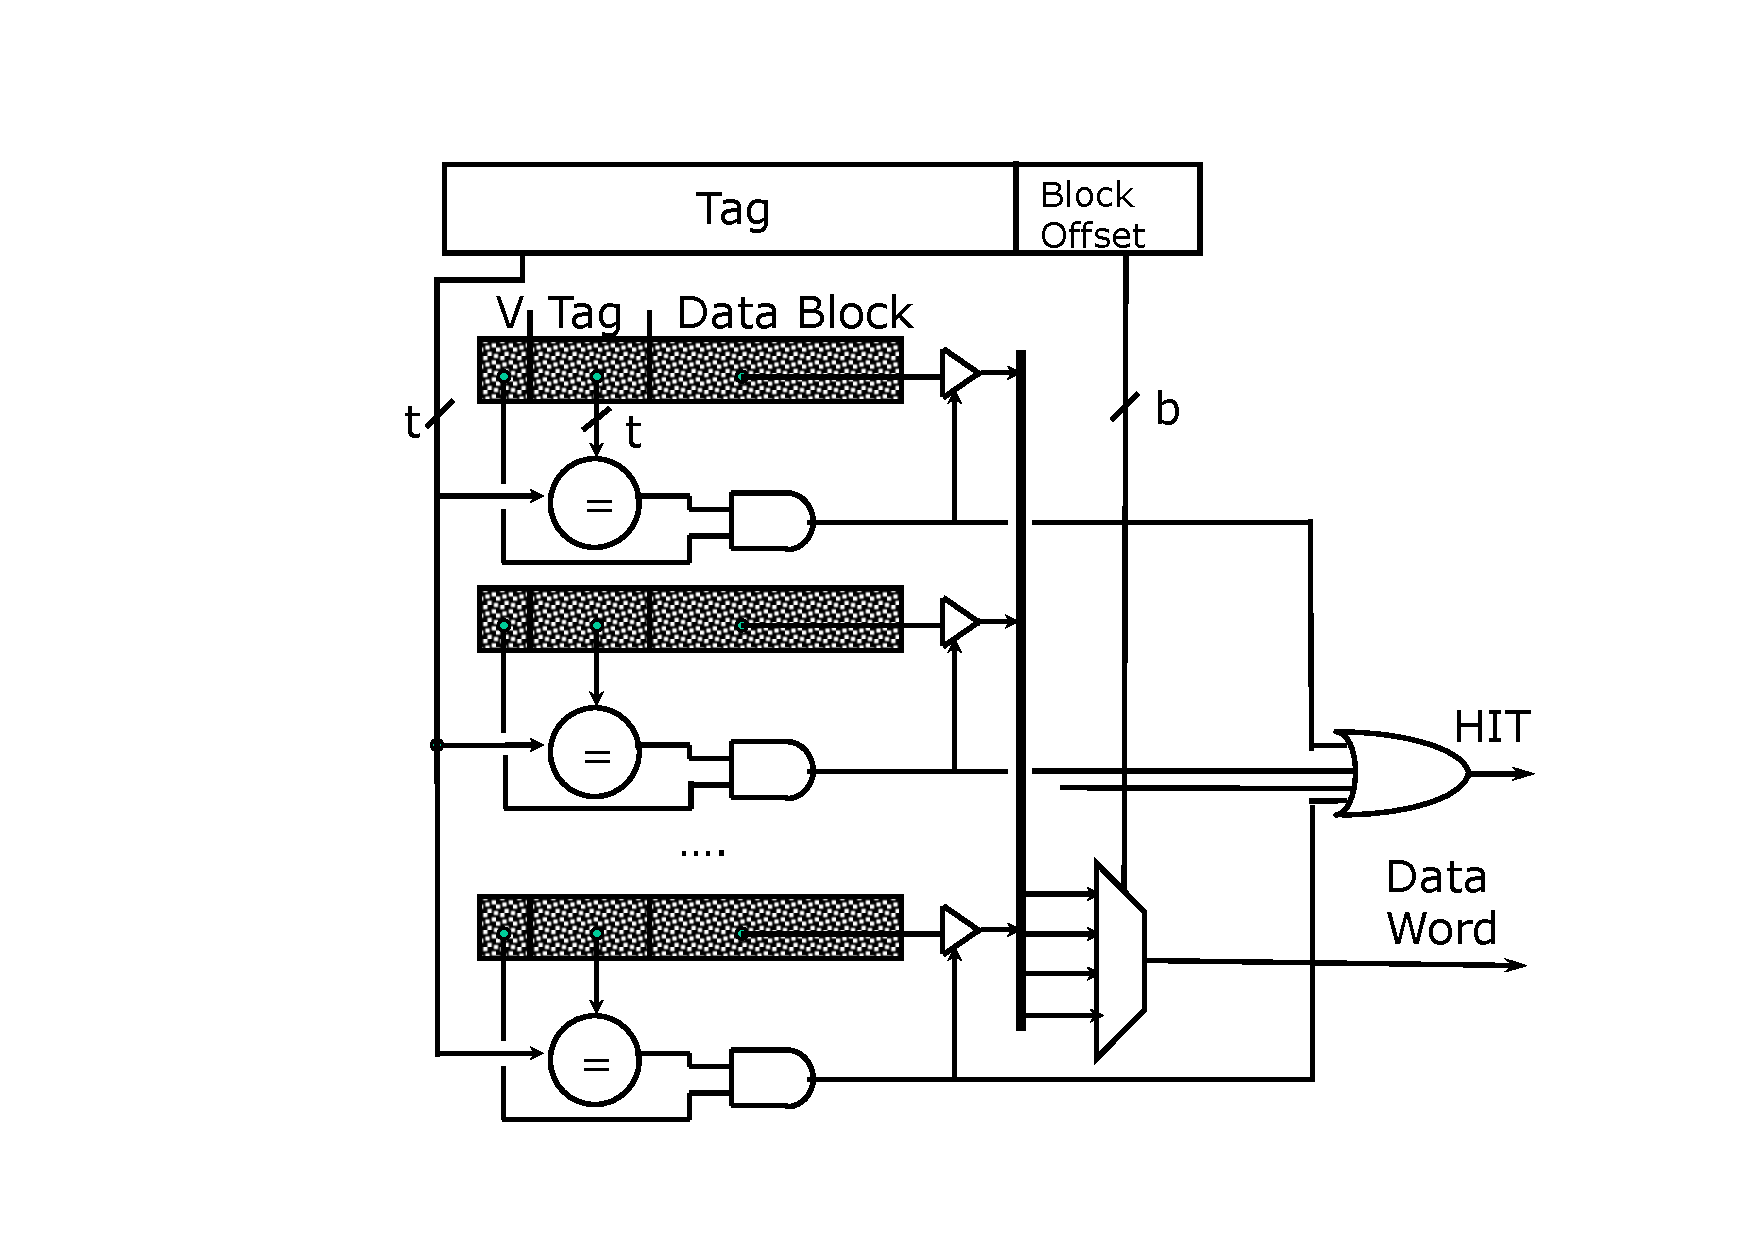
\includegraphics[width=.7\textwidth]{img/fully-associative-cache-2.pdf}
    \caption{The cache structure of the \emph{Fully Associative Cache} technique.}
    \label{fig: cache structure of the Fully Associative Cache}
\end{figure}

\noindent
As shown in Figure~\ref{fig: cache structure of the Fully Associative Cache}, the cache structure is more accessible because there are no \emph{Index} fields. We check only the \emph{Tag} field from the memory address. Finally, the \emph{Block Offset} chooses the \emph{Data Block} from the cache. We have a cache hit if the \emph{Tag} is equal to the \emph{Tag} of the cache and the value in and with the valid bit is true.

\newpage

\noindent
For \example{example}, we assume a block-frame address composed of 32 bits. Our cache structure is fully associative, and the number of cache blocks is 8. A possible exercise could be \textbf{determining where block 12 can be placed in the 8-block cache}.

\highspace
Unlike before, the position can be anywhere.

\begin{figure}[!htp]
    \centering
    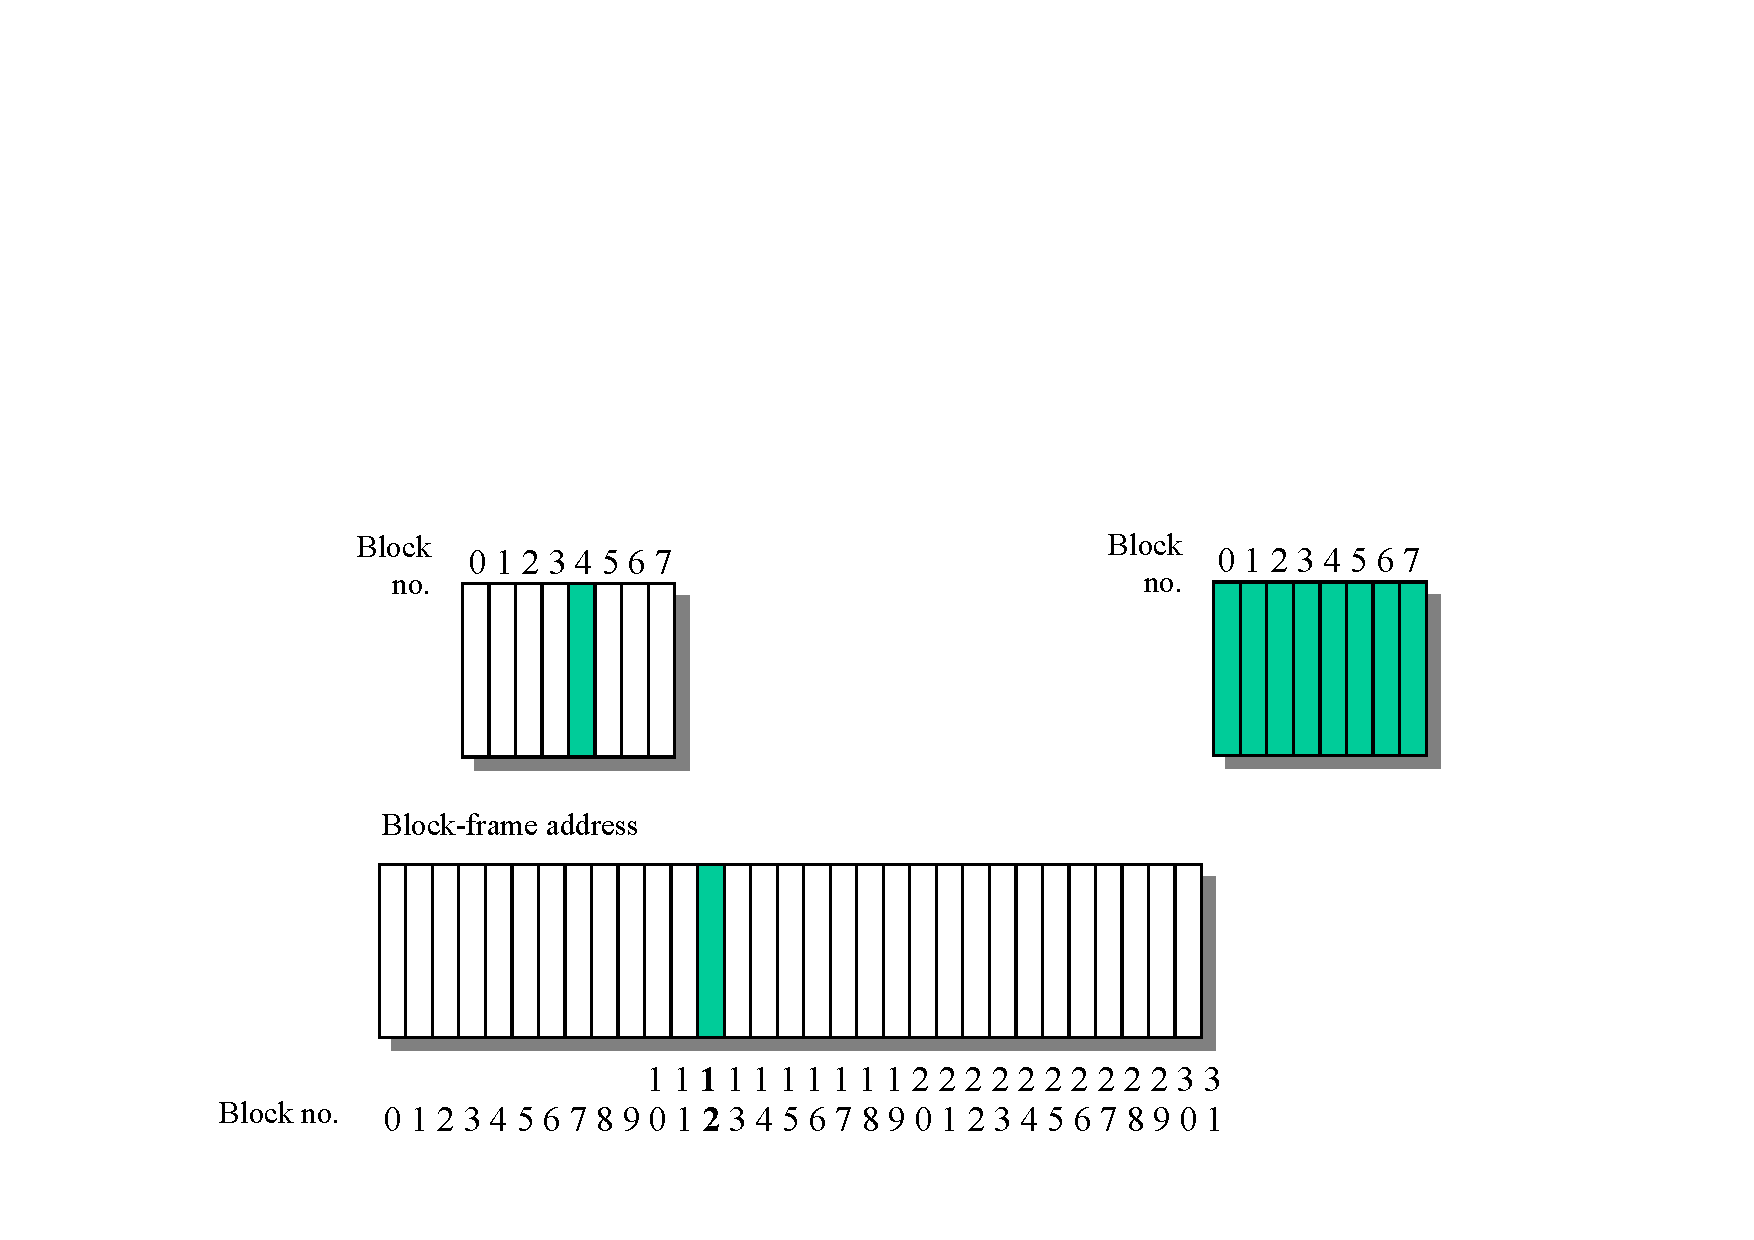
\includegraphics[width=.8\textwidth]{img/fully-associative-cache-3.pdf}
    \caption*{Direct Mapped on the left and Fully Associative on the right.}
\end{figure}

\newpage

\subsubsection*{\textcolor{Red2}{\emph{n}-way Set-Associative Cache}}\label{n-way Set-Associative Cache}

In a \definition{\emph{n}-way Set Associative Cache}, the \textbf{cache is composed of sets}. Each set is composed of \emph{n} blocks:
\begin{equation}
    \begin{array}{rcl}
        \texttt{Number of blocks} &=& \dfrac{\texttt{Cache Size}}{\texttt{Block Size}} \\ [1.5em]
        \texttt{Number of sets} &=& \dfrac{\texttt{Cache Size}}{\left(\texttt{Block Size} \times n\right)}
    \end{array}
\end{equation}
The memory block can be placed in any block of the set, so the \emph{search must be done on all the blocks}.

\highspace
\textbf{Each memory block corresponds to a single set of the cache}, and the \textbf{block can be placed in whatever block of the \emph{n} blocks of the set}:
\begin{equation}\label{eq: set cache}
    \left(\texttt{Set}\right)_{\texttt{cache}} = \left(\texttt{Block address}\right)_{\texttt{mem}} \texttt{mod} \left(\texttt{\# sets in cache}\right)
\end{equation}

\begin{figure}[!htp]
    \centering
    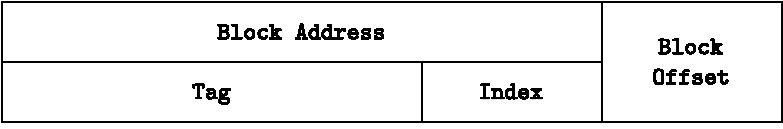
\includegraphics[width=\textwidth]{img/direct-mapped-cache-1.pdf}
    \caption{The memory address comprises the block address (Tag and index used to identify the set) and the block offset.}
\end{figure}

\begin{figure}[!htp]
    \centering
    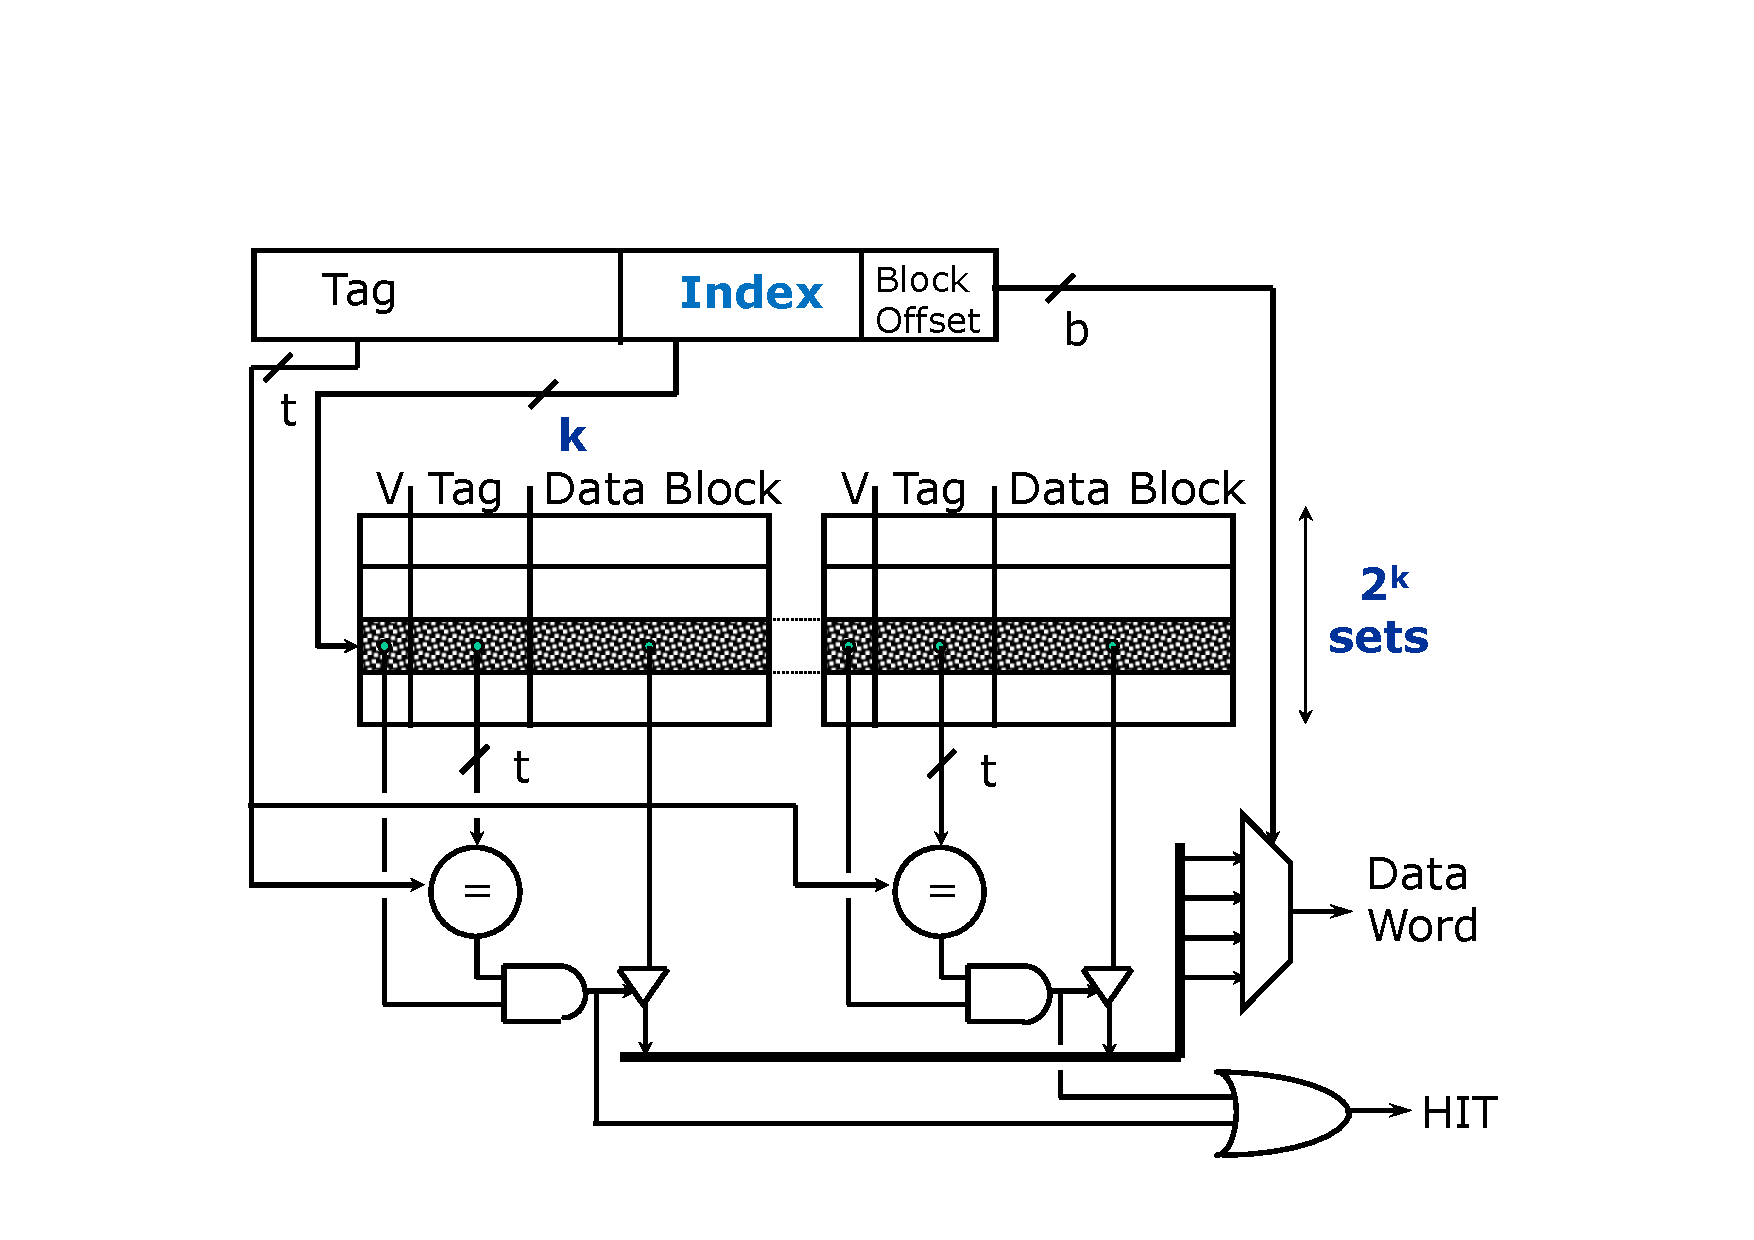
\includegraphics[width=.7\textwidth]{img/n-way-set-associative-cache-1.pdf}
    \caption{This structure is a \textbf{2-way Set Associative Cache}.}
\end{figure}

\newpage

\noindent
Taking the \example{examples} of previous pages, with the 2-way Set Associative, the answer is anywhere in set $0$. The reason for this is that using the formula~\ref{eq: set cache}:
\begin{equation*}
    \left(\texttt{Set}\right)_{\texttt{cache}} = 12 \mod 4 = 0
\end{equation*}

\begin{figure}[!htp]
    \centering
    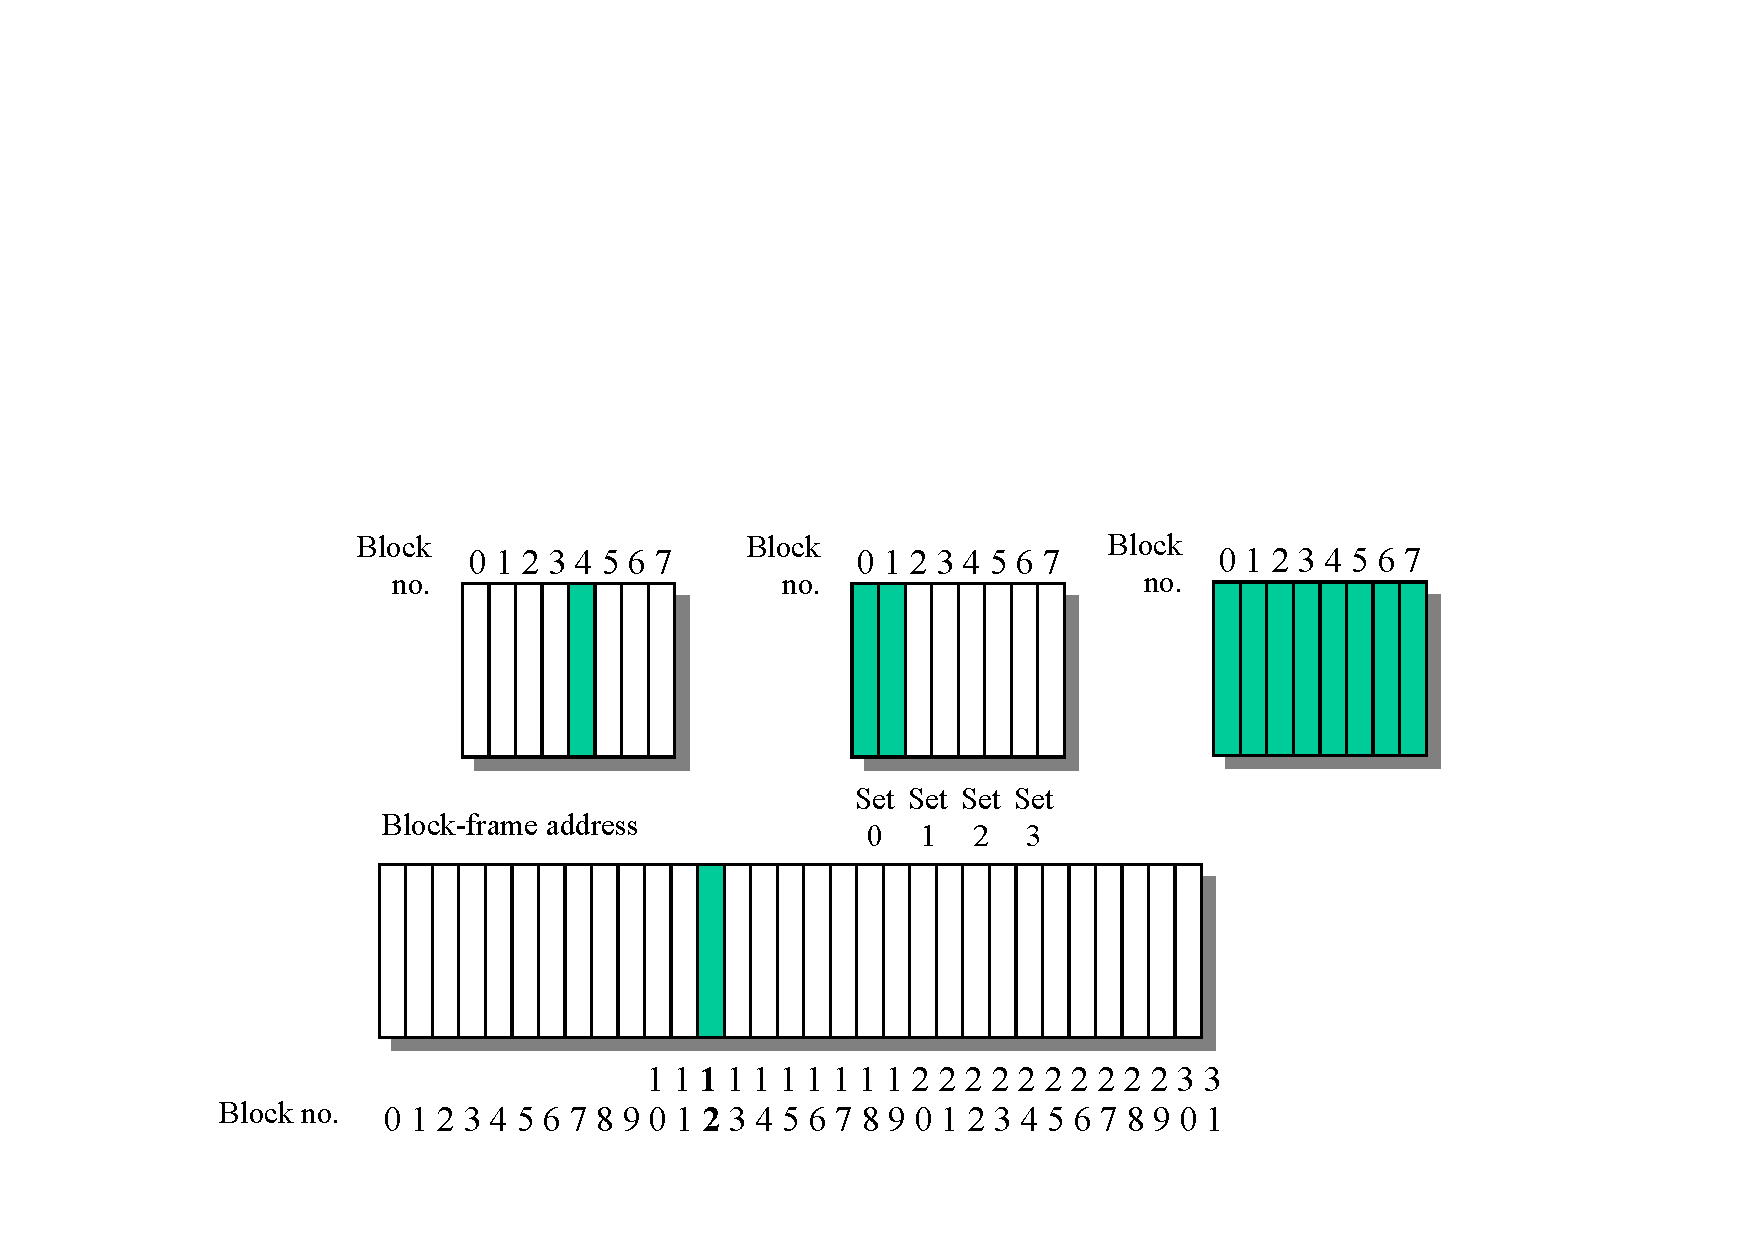
\includegraphics[width=\textwidth]{img/n-way-set-associative-cache-2.pdf}
    \caption*{Direct Mapped on the left, 2-way Set Associative on the center and Fully Associative on the right.}
\end{figure}